\cotefile{130}
\scanpage{2}
\hfill \unsure{Formule|Formules} de Néron
% archive sheet number: 1
\scanpage{4}
\begin{center}\uline{Formules de Néron}\end{center}

$A_K$ V.A. sur $K$ corps des fractions de $V$, anneau
de val. discrète (corps résiduel fini \unsure{\}|?} ?)

On définit une fonction $\unsure{v|\nu}(X,\underline a)$ \inserted{à valeurs dans $\mathbb Q$} sur la partie
de $D_a(\deleted{\unsure{A}}A_K)\times\unsure{\mathfrak Z|Z}_0^*(A_K)\deleted{\unsure{K}}$ formée des couples $X,\underline a$ tels
que $\operatorname{supp}X\cap\operatorname{supp}\underline a=\varnothing$, uniquement déterminée
par les propriétés suivantes :

(i) bilinéaire.

(ii) Invariant par translation par les $a\in A(K)$

(iii) Si $X\underset{\ell}{\sim}0$, \deleted{Alors} \deleted{et} $X=\operatorname{div}(f)$, on a

\[
 v(X,\underline a)=\sum_{x_0\in A_0}i(\deleted{\unsure{\overline{\phantom{x}}}}\operatorname{div}_{\unsure{s_0|f_0|g}}(\bar f),\overline{\underline a}\,;x_0)
\]

% slanted
\margin{Si $m=1$ i.e. $A_0$ connexe, \uline{alors} $v(X,\underline a)=0$ si $X\underset{\rm alg}{\sim}0$ et par \unsure{suite|vraiment} $v(X,\underline a)_V=0$ pour \unsure{tt|$\forall$} $X,\underline a$}

$A$ est le \uline{modèle de Néron} de $A$, $A_0
=A\otimes_V k$, $\bar f$ est $f$ considérée comme fonction sur $A$,
\deleted{et} $\operatorname{div}_{s_0}\bar f$ est la composante verticale de $\operatorname{div}(\bar f)$,
$\overline{\underline a}$ est l’``adhérence'' de $\underline a$ dans $A$. \}

(iv) Pour $X\in D_a(A_K)$ fixé, $0\notin\operatorname{supp}X$, et
$x\in A(K)$, $x\notin\operatorname{supp}X$ variable, $v(X,(x)-(0))$ est
borné.

De plus, on a les propriétés suivantes :

(iv bis) $v(X,(x)-(a))$ ne dépend (pour $X\in D_a(A_K)$
\deleted{fixé, on} et $a\in A(K)$, $a\notin\operatorname{supp}X$ fixés) \deleted{$x$ variable}
que de la classe de $x$ mod $A(K)^0={}$Im. inv. de $A_0^0(\unsure{k})$
donc ne prend qu’un nb fini de valeurs.
% archive sheet number: 3
\scanpage{5}
(v) Si $X\in D_\ell(A_K)$ \uline{ou} $\underline a\in Z_\ell^{\unsure{*|'}}(A_K)$, on a
$\unsure{v|\nu}(X,\underline a)\in\mathbb Z$.

% slanted
\margin{\deleted{\unsure{pour} $X$, \illegible{1} $\underline a$ \unsure{fixés}, \illegible{1} \unsure{ne dépend}}}

(vi) Si $m={}\text{degré de }A_0/A_0^0$, alors on a
tjrs $m v(X,\underline a)\in\mathbb Z$.

[N.B. On obtient donc \inserted{par (v) et (vi)} un accouplement remarquable

\[
\underset{\substack{\shortparallel\\ A^*(K)}}{D_a(A_K)/D_\ell(A_K)}
 \times Z_0^*(A_K)/Z_\ell^*(A_K)\longrightarrow
 \underset{\substack{\shortparallel\\ {}_m(\mathbb Q/\mathbb Z)}}{\mathbb Z/m\mathbb Z}
\]

% slanted
\margin{À examiner : Cas d’un fibré principal homogène sous une VA \unsure{$\downarrow$|et}}

\deleted{pour \unsure{une} \unsure{valeur|unicité} \unsure{$0)$|$?)$}} par suite

\[
 A^*(K)\times A(K)\longrightarrow\mathbb Z/m\mathbb Z \qquad ]\tag*{$*$}
\]

La relation avec le symbole local $(X,\underline a)_v$ est
donnée par

\[
 \boxed{(X,\underline a)_v=v(X,\underline a)+\sum_{x_0\in A_0^{\unsure{*|c}}}i(\bar X\unsure{,|\,\cdot\,}\overline{\underline a},x_0)}\tag*{(vii)}
\]

% slanted
\margin{Se généralise aussitôt à des variétés quelconques \textendash\textendash\textendash}

Ceci montre que $(X,\underline a)_v\in\frac{1}{m}\mathbb Z$ pour tt $X,\underline a$,
\deleted{donc} à fortiori il est \uline{rationnel}, et il est
entier si $X\in D_\ell(A_K)$ [On le savait
déjà, car on trouve, si $X=\operatorname{div} f$, $(X,\underline a)_v=v(f(\underline a))$]
\uline{ou} si $\underline a\in\deleted{\unsure{D}}Z_\ell^*(A_K)$. On trouve donc
% archive sheet number: 4
\scanpage{6}
une \deleted{autre} \inserted{expression de l’}accouplement $*$ en termes
de $(X,\underline a)_v$. \deleted{On voit \unsure{s|q}}

\[
 \text{\uline{Cor}}\quad\unsure{v|\nu}(X_{\underline a},\underline b)=v(X_{\underline b}^{-},\underline a)\quad(=v(X_{b^{-}},\underline a^{-}))
\]

Dans le cas global [où on a une
famille de \uline{valuations} \uline{discrètes} satisfaisant la
formule du produit], on obtient un
accouplement\deleted{\unsure{aux}} $D_a^{\unsure{*}}(A_K)\times\deleted{\unsure{D}}Z_0^*(A_K)\longrightarrow\mathbb R$
par \deleted{produit} produit des symboles locaux

\[
 (X,\underline a)=\sum_v(X,\underline a)_v
\]

qui ne dépend plus que des classes \deleted{de}
mod $D_\ell(A_K)$ resp. mod $Z_\ell^*(A_K)$, et définit
donc un accouplement

\[
 A^*(K)\times A^{\deleted{\unsure{*}}}(K)\longrightarrow\mathbb R .
\]

On obtient donc : cet accouplement est
à valeurs dans $\frac1m\mathbb Z\subset\mathbb Q$, où
$m$ est un entier $>0$ convenable

La forme en question est la \uline{forme de
Néron-Tate}. \deleted{Elle est \unsure{multipliée|multiplicative}}
% archive sheet number: 5
\scanpage{7}
$X\xrightarrow{f}S$ morphisme \deleted{régulier} propre

$X$ régulier

$S$ régulier. irréductible, pt. gén. $\eta$

On suppose que $\underline{\operatorname{Pic}}_{X/S}^{\deleted{\unsure{0}}}$ existe, et \deleted{est une V.A.}
\deleted{Par} que l’adhérence \inserted{schématique} de $A_\eta=\underline{\operatorname{Pic}}_{X_\eta/k(\eta)}^{0}$, \deleted{\unsure{est}}\unsure{soit} un
\uline{sous-schéma en groupes} \uline{plat} de $X$, \deleted{ce qui}
\uline{lisse} sur $S$ \deleted{\unsure{a|\textemdash}} ce qui est automatiquement
le cas si $\underline{\operatorname{Pic}}^{\unsure{0}}_{X/S}$ est lisse sur $S$ le long de
la section unité, p.ex. si $S$ régulier de dim $1$
et les $\operatorname{Pic}_{X_s/k(s)}$ sont lisses $s\in S$).

Alors \deleted{$\operatorname{Pic}$} $A$ \uline{est un modèle de Néron} :
en effet, si $S'/S$ est lisse, alors
$X'=X\times_S S'$ est lisse sur $X$ régulier, donc est
régulier, donc tt \deleted{\unsure{sectio|section}} élément de $\operatorname{Pic}(X'_{\unsure{\eta'|\eta}})$
provient d’un élément de $\operatorname{Pic}(X')$.

% slanted
\margin{Attention s’il n’y a pas de section locale \inserted{(ét.)} de $X$ sur $S$}
% archive sheet number: 6
\scanpage{8}
\hfill\handwritten{\unsure{Ag|AG}}

% slanted
\margin{\handwritten{Matrices de Coxeter\\ \unsure{Matrice|Matrices} de Cartan\\ Systèmes de racines\\ groupes engendrés par des \unsure{réflexions}\\ diagrammes de Dynkin}}

\begin{center}GRIE ET ALGOUPES DE LEBRES.\hfill N\textsuperscript{o}383\end{center}

\begin{center}CHAPITRE III.\end{center}

\begin{center}SYSTINES DE RACEMES (Etat 3).\end{center}

\begin{center}\mbox{-{}-{}-{}-{}-{}-{}-{}-{}-{}-{}-{}-}\end{center}

\begin{center}\uline{Sommaire}\end{center}

\begin{center}\S~1. \uuline{Résultats préliminaires}.\end{center}

1. Lemmes sur les chambres \dotfill{} 1

2. Lemmes sur les espaces hilbertiens réels de dimension finie \dotfill{} 3

3. Lemmes de Géométrie plane \dotfill{} 5

\begin{center}\S~2. \uuline{Groupes de Coxeter}.\end{center}

1. Définition des groupes de Coxeter \dotfill{} 1

2. Représentation directe d’un groupe de Coxeter \dotfill{} 3

3. Représentation contragrédiente d’un groupe de Coxeter \dotfill{} 5

4. Démonstration du théorème 2 \dotfill{} 8

5. La réunion des chambres \dotfill{} 15

6. Critère de finitude d’un groupe de Coxeter \dotfill{} 16

\begin{center}\S~3. \uuline{Groupes engendrés par des réflexions}.\end{center}

1. Groupes finis engendrés par des réflexions vectorielles \dotfill{} 1

2. Groupes affines engendrés par des réflexions \dotfill{} 6

3. Points spéciaux \dotfill{} 13

\begin{center}\S~4. \uuline{Systèmes de racines}.\end{center}

1. Définition d’un système de racines \dotfill{} 1

2. Relations entre deux racines \dotfill{} 5

3. Systèmes de racines réduits \dotfill{} 9

4. Chambres. Racines positives. Racines simples \dotfill{} 11

5. Plus grande racine \dotfill{} 13

6. Ensembles clos de racines \dotfill{} 13

7. Groupes commutatifs libres définis par un système de racines \dotfill{} 17
% archive sheet number: 7
\scanpage{10}
$X$ surface \inserted{n’est pas une restriction essentielle ! $\dim X\geq 2$} algébrique projective non singulière conn.
sur $k$ alg. clos.

$Y_0$ section hyperplane non singulière, dans un
``pencil'' défini par $L^{n-2}\subset P^n$ coupant $X$
transversalement en $Z$

$\widetilde X$ \unsure{obtenue|obtenu} en faisant éclater $Z$

\diagram{\begin{tikzcd}[ampersand replacement=\&]
X \& \widetilde X\arrow[l,"\varphi"']\arrow[d] \& \widetilde Y_{\bar\eta}\\
\deleted{\downarrow} \& \mathbb P^1 \&
\end{tikzcd}}

\diagram{\begin{tikzcd}[ampersand replacement=\&]
\operatorname{Pic}(X)\arrow[r,hook]\arrow[dr] \& \operatorname{Pic}(\widetilde X)\arrow[d]\\
\& \operatorname{Pic}(\widetilde Y_{\overset{\deleted{-}}{\eta}})
\end{tikzcd}}

Soit $\operatorname{Pic}(X)'$ ($\operatorname{Pic}(\widetilde X)'$) le sous-groupe des
\deleted{diviseurs} classes induisant sur $\widetilde Y_{\bar\eta}$ une classe
de \uline{degré} $0$. On a donc

\diagram{\begin{tikzcd}[ampersand replacement=\&]
\operatorname{Pic}(X^{\deleted{\unsure{'|*}}})'\arrow[r,hook]\arrow[dr] \& \operatorname{Pic}(\widetilde X)'\arrow[d]\\
\& \operatorname{Pic}^0(\widetilde X_{\bar\eta})=J^0(\widetilde X_{\bar\eta})
\end{tikzcd}}
% archive sheet number: 9
\scanpage{11}
\figure{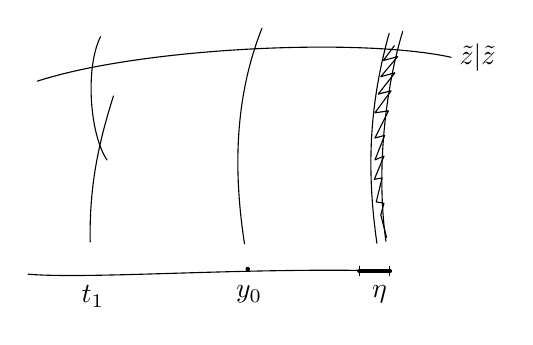
\begin{tikzpicture}[x=.82cm,y=.82cm,line cap=round,line join=round]
\draw (0,0) .. controls (1,-.08) and (3.4,.11) .. (5.60,.05);
\draw[line width=1.7pt] (5.13,.05)--(5.60,.05);
\draw (5.13,-.02)--(5.13,.12) (5.60,-.02)--(5.60,.12);
\fill (3.40,.08) circle (.035);
\node[below] at (1.00,-.03) {$t_1$};
\node[below] at (3.42,-.03) {$y_0$};
\node[below] at (5.44,-.03) {$\eta$};
\draw (.96,.50) .. controls (.94,1.42) and (1.12,2.13) .. (1.32,2.76);
\draw (1.22,1.77) .. controls (.95,2.17) and (.88,3.20) .. (1.12,3.68);
\draw (3.35,.47) .. controls (3.15,1.76) and (3.24,2.85) .. (3.62,3.81);
\draw (5.40,.48) .. controls (5.25,1.54) and (5.26,2.55) .. (5.59,3.73);
\draw (5.54,.51) .. controls (5.37,1.71) and (5.57,3.02) .. (5.80,3.76);
\draw (5.55,.57)--(5.46,.92)--(5.51,1.10)--(5.39,1.12)--(5.48,1.49)--(5.36,1.47)--(5.51,1.83)--(5.37,1.77)--(5.52,2.15)--(5.37,2.11)--(5.58,2.53)--(5.37,2.50)--(5.62,2.84)--(5.42,2.79)--(5.68,3.12)--(5.46,3.06)--(5.72,3.37)--(5.50,3.31)--(5.67,3.54);
\draw (.14,2.99) .. controls (1.74,3.51) and (5.14,3.67) .. (6.55,3.36);
\node[right] at (6.53,3.36) {$\unsure{\tilde z|\tilde{\mathfrak z}}$};
\end{tikzpicture}}

À déterminer a) les noyaux de
\diagram{\begin{tikzcd}[ampersand replacement=\&,row sep=0pt,column sep=2.2em]
\operatorname{Pic}(X^{\unsure{+|'|*}})'\arrow[r] \& \raisebox{-.7ex}{$\deleted{\operatorname{Pic}}J^0(\widetilde X_{\bar\eta})$}\\
\operatorname{Pic}(\widetilde X)'\arrow[r,phantom,"\unsure{\text{---}|\longrightarrow}" description] \& {}
\end{tikzcd}}

b) leur image

\uline{N.B.} $\operatorname{Pic}(\widetilde X_\eta)\longrightarrow\operatorname{Pic}(\widetilde X_{\bar\eta})$ est injectif, donc
le noyau de $\operatorname{Pic}(\widetilde X)^{\deleted{\unsure{'|*}}}\text{---}\operatorname{Pic}(\widetilde X_{\bar\eta})$ \deleted{\illegible{2}}
(égal au noyau de $\operatorname{Pic}(\widetilde X)'\text{---}J^0(\widetilde X_{\bar\eta})$) est
aussi celui de $\operatorname{Pic}(\widetilde X)\text{---}\operatorname{Pic}(\widetilde X_\eta)$, ie
est formé des \uline{classes des diviseurs verticaux}

\deleted{Parmi ceux-ci,} Noter que les div.
verticaux $\widetilde X_y$, pour $y\in\mathbb P^1(k)$, \deleted{($\widetilde X_y$ non \unsure{sing.})}
sont lin. équivalents entre eux, donc à
$\widetilde X_{y_0}=\widetilde Y_0\simeq Y_0$. \deleted{\unsure{Partant|Donc}} Si \inserted{\uline{tous}} les $X_y$ sont \deleted{irr. et}
\deleted{\unsure{div.} \unsure{ver.}} \uline{intègres}, alors le noyau de
$\operatorname{Pic}(\widetilde X)'\longrightarrow\deleted{\operatorname{Pic}}J^0(\widetilde X_{\bar\eta})$ est réduit aux \deleted{classes des} multiples
de \deleted{$\operatorname{cl}(\widetilde X_y)$} la classe \deleted{$\unsure{\widetilde X_y}$} de $\widetilde Y_0$, \deleted{\unsure{Notons} \unsure{pour|que}} \inserted{soit $\tilde\xi_0$}, qui est
% archive sheet number: 10
\scanpage{12}
égal à $\varphi^*(\unsure{\xi_0|\varphi_0})-\sum_{z\in Z}\tilde z_{\unsure{\ell|z}}$, où $\xi_0$ est la classe de
$Y_0$ dans $X$. Par suite, \deleted{si} \inserted{comme} $Z\ne\varnothing$, on
a $n\in\mathbb Z$, $n\ne0\Longrightarrow n\tilde\xi_0\notin\operatorname{Pic}(X)'$. Donc
dans le cas envisagé, $\operatorname{Pic}(X)^{\deleted{\unsure{'}}}\longrightarrow\operatorname{Pic}(\widetilde X_{\bar\eta})=\operatorname{Pic}(Y_{\bar\eta})$
est \uline{injectif}.

L’image de $\operatorname{Pic}^0(X)\simeq\operatorname{Pic}^0(\widetilde X)$ dans
\deleted{$\operatorname{Pic}(\widetilde X_{\bar\eta}$} $\operatorname{Pic}^0(Y_{\bar\eta})=J(Y_{\bar\eta})(k)$ est la ``partie \deleted{\unsure{f}} fixe''
$J(Y_{\bar\eta})^{\mathrm{fixe}}(\deleted{\unsure{k(\bar\eta)|k}})$ et de façon précise on a \deleted{des} isos

\[
\operatorname{Pic}^0(X)\xrightarrow{\sim}\operatorname{Pic}^0(\widetilde X)\xrightarrow{\sim}
\underset{\substack{\shortparallel\\ \deleted{\operatorname{Pic}}J(Y_{\bar\eta})^{\rm fixe}(k(\eta))}}
{\deleted{\operatorname{Pic}}J(Y_{\bar\eta})^{\rm fixe}(k)\deleted{\unsure{(\eta)}}}
\]

[N.B. \deleted{\unsure{$k(\eta)$}} $k(\eta)$ est
une extension \uline{pure} de $k(\eta)$, donc pour tte
V.A. $A$ sur $k$, $A(k)\simeq A(k(\eta))$]. On obtient
alors

\diagram{\begin{tikzcd}[ampersand replacement=\&]
\mathrm{NS}(X)'\arrow[r,hook] \& \mathrm{NS}(\widetilde X)'\arrow[d]\\
\& J'(k(\eta))
\end{tikzcd}}

où $J'=J/J^{\rm fixe}_{k(\eta)}$ est ``la partie mobile'' de $J=
J(Y_\eta/k(\eta))$. Notons que le noyau de
% archive sheet number: 11
\scanpage{13}
$\mathrm{NS}(\widetilde X)'\longrightarrow J'(k(\eta))$ est égal au groupe engendré
par l’image de $\tilde\xi_0$, car si $\alpha$ est
dans le noyau, alors $\alpha$ provient de
$\alpha_0\in\operatorname{Pic}(\widetilde X)'$, et comme p.h. l’image de
$\alpha_0$ dans $\deleted{\unsure{\operatorname{Pic}}}J(Y_\eta)$ est dans $J(Y_\eta)^{\rm fixe}\simeq\operatorname{Pic}^0(\widetilde X)$,
il s’ensuit que quitte à modifier $\alpha_0$ par
un \unsure{élmt|élément} de $\operatorname{Pic}^0(\widetilde X)$, on aura une
image nulle \ldots{} Donc sous réserve
que tous les $Y_y$ soient intègres, le
noyau de $\mathrm{NS}(\widetilde X)'\unsure{\text{---}|\longrightarrow}J'(k(\eta))$ est
de rang $1$, et engendré par l’image de $\bar\xi_0$.

Enfin, je dis que \deleted{l’image de} $\mathrm{NS}(\widetilde X)'\longrightarrow J'(k(\eta))$
est \uline{surjectif} \inserted{mod groupe fini}. En effet, \deleted{un élément de
$J'(k(\eta))$} comme $H^1(K,J'')$ est un
groupe de torsion \unsure{[|$T$} où $K=k(\eta)=k(t)$,
$J''=J^{\rm fixe}$) on voit que mod groupes finis,
\deleted{$\mathrm{NS}(\widetilde X)'\text{---}J'(k(\eta))$ \unsure{v|est}} $J(k(\eta))\text{---}J'(k(\eta))$ est
surjectif, donc il suffit de prouver
que $\operatorname{Pic}(\widetilde X)'\longrightarrow J(k(\eta))$ est surjectif \deleted{\unsure{mod}}
% archive sheet number: 12
\scanpage{14}
\deleted{à un \unsure{gpe|groupe} fini.} Or un élément de
$J(k(\eta))$ \deleted{\unsure{provi|qui}} provient \deleted{\unsure{peut} \unsure{être} \unsure{de la} \unsure{une}
obstruction de \unsure{t}} d’une classe de
\unsure{diviseur|diviseurs} de degré $0$ sur $Y_\eta$

[N.B. le groupe de Brauer de $k(\eta)=k(\unsure{s|t})$
est nul, par Tsen] et on gagne

\[
 \boxed{\rho(\widetilde X)-1=}\boxed{\rho(X)+z-2=\rho(J')}.
\]

\[
\left\{\begin{aligned}
&\rho(X)\quad\text{nb de Picard de }X\\
&z=\text{nb de sections singulières du pinceau}\\
&\rho(J')\quad\deleted{\unsure{\mathrm{nb}|=}}\ \text{rang du groupe des pts rat. sur }k(\eta)\\
&\hspace{3em}\text{de }J'=J(X_\eta)/J(X_\eta)^{\rm fixe}
\end{aligned}\right.
\]

Condition de validité de la formule :
toutes les sections du pinceau sont \deleted{intègres.}
\uline{irréductibles} (intègre n’est pas absolument \unsure{néc|néc.},
i.e. on admet des sections multiples \ldots).
% archive sheet number: 13
\scanpage{15}
Supposons $X$ une \uline{surface}.

Notons maintenant que $J'$ a une polarisation
canonique, héritée de celle de $J$. \deleted{\unsure{Soit|Car} $J'_0$
une sous [En effet, \unsure{la|le} \unsure{du|dual de} $J$ étant sa
$J\to$ propre duale, $\unsure{\check J'|J'|\hat J'}$ la duale de $J'$ se plonge
canoniquement dans $J$, donc hérite une
polarisation, d’où une polarisation}

On en conclut \inserted{par Néron-Tate} une forme quadratique
canonique \deleted{\unsure{sur}} définie positive \inserted{$Q$} sur $J'(k(\eta))$.

D’autre part, il y a \deleted{aussi} une forme
quadratique définie négative sur $\mathrm{NS}(X)'$
savoir la forme intersection.

\margin{$i\deleted{\unsure{\xi}}:\mathrm{NS}(X)'\longrightarrow J'(k(\eta))$}

À prouver la formule

\margin{?}

\[
 \boxed{Q(i(\unsure{\xi|\zeta}),i(\eta))=-\deleted{\unsure{\xi}}\xi\cdot\eta}
 \qquad(\xi,\eta\in\mathrm{NS}(X)')
\]

valable si les $Y_t$ sont tous \uline{intègres} ?
% archive sheet number: 14
\scanpage{17}
1) $f:X\longrightarrow S$ projectif, $X$ régulier,
$S$ \unsure{spectr.|spectre,|spectre} ann. de val. discrète
pt générique $\eta$, pt spécial $s$

\[
\left\{\begin{aligned}
&X_\eta \text{ est lisse}\\
&X_s \text{ est géom\textsuperscript{t} intègre }\deleted{\unsure{\text{algébr.}}}
\end{aligned}\right.
\]

\[
 \unsure{\Longleftrightarrow|\Longrightarrow|\text{\deleted{Soit}}}\quad\dim X_\eta=n\qquad\dim X=n+1
\]

$C,D$ deux cycles sur $X$, de codimensions
$c$ et $d$ avec $c+d=n+1$. On suppose

a) \deleted{\illegible{1}} $C_\eta$ et $D_\eta$ sont alg. équiv. à $0$
\deleted{\unsure{et} et $\operatorname{supp}C_\eta\cap\operatorname{supp}D_\eta=\varnothing$}

b) $C$ et $D$ \unsure{n’aient|n’ont} que des \unsure{composants|composantes} \unsure{horizontales|horizontaux|horizontal},
i.e. $C=\overline{C_\eta}$, $D=\overline{D_\eta}$.

c) $C.D$ est défini $[\Longrightarrow\operatorname{supp}C_\eta\cap\operatorname{supp}D_\eta=\varnothing]$

Considérons $i(C.D)$, il ne dépend que de
$C_\eta$ et $D_\eta$, cycles \deleted{alg.} de $X_\eta$ \inserted{alg. équ. à $0$} de codimensions
$c,d$ tels que $c+d=n+1$, \deleted{On veut} \inserted{de supports}
disjoints. On veut alors donner une
description de $i(C.D)$ en termes
de $C_\eta,D_\eta$, comme un

\[
 \langle C_\eta,D_\eta\rangle_v
\]

\uline{indépendant du modèle $X$} \inserted{\uline{ou de son existence}},
(\uline{à valeurs dans $\mathbb Q$} \inserted{à priori})
% archive sheet number: 16
\scanpage{18}\mspage{-VII- 10 -}
% Faint mark at upper right, possibly showing through from the other side.
\margin{\handwritten{\unsure{XV|XY}}}
\hfill n\textsuperscript{o}383

est l'ensemble des transformés des $u_i$ (resp. $u'_i$) par $G$ (resp. $G'$) (\S~4, n\textsuperscript{o}4, prop.5),
de sorte que $f(S)=S'$. C.Q.F.D.

THEOREME 2.- \uline{Les schémas de Dynkin des systèmes de racines réduits irréductibles
sont à choisir}, \uline{à une homothétie près sur les coefficients}, \uline{parmi les schémas
suivants} :

\diagram{\begin{tikzcd}[ampersand replacement=\&,column sep=1.25em,row sep=.45em]
A_r \& |[inner sep=0pt,label=above:{\scriptsize $1$}]|{\scriptstyle\vert}\arrow[r,dash] \& |[inner sep=0pt,label=above:{\scriptsize $1$}]|{\scriptstyle\vert}\arrow[r,dash] \& |[inner sep=0pt,label=above:{\scriptsize $1$}]|{\scriptstyle\vert}\arrow[r,dash,dashed] \& |[inner sep=0pt,label=above:{\scriptsize $1$}]|{\scriptstyle\vert}\arrow[r,dash] \& |[inner sep=0pt,label=above:{\scriptsize $1$}]|{\scriptstyle\vert}\arrow[r,dash] \& |[inner sep=0pt,label=above:{\scriptsize $1$}]|{\scriptstyle\vert} \& (r\handwritten{\geq}1\text{ noeuds})
\end{tikzcd}}

\diagram{\begin{tikzcd}[ampersand replacement=\&,column sep=1.25em,row sep=.45em]
B_r \& |[inner sep=0pt,label=above:{\scriptsize $1$}]|{\scriptstyle\vert}\arrow[r,dash] \& |[inner sep=0pt,label=above:{\scriptsize $1$}]|{\scriptstyle\vert}\arrow[r,dash] \& |[inner sep=0pt,label=above:{\scriptsize $1$}]|{\scriptstyle\vert}\arrow[r,dash,dashed] \& |[inner sep=0pt,label=above:{\scriptsize $1$}]|{\scriptstyle\vert}\arrow[r,dash] \& |[inner sep=0pt,label=above:{\scriptsize $1$}]|{\scriptstyle\vert}\arrow[r,dash] \& |[inner sep=0pt,label=above:{\scriptsize $(1/2)$}]|{\scriptstyle\vert} \& (r\handwritten{\geq}1\text{ noeuds})
\end{tikzcd}}

\diagram{\begin{tikzcd}[ampersand replacement=\&,column sep=1.25em,row sep=.45em]
C_r \& |[inner sep=0pt,label=above:{\scriptsize $1$}]|{\scriptstyle\vert}\arrow[r,dash] \& |[inner sep=0pt,label=above:{\scriptsize $1$}]|{\scriptstyle\vert}\arrow[r,dash] \& |[inner sep=0pt,label=above:{\scriptsize $1$}]|{\scriptstyle\vert}\arrow[r,dash,dashed] \& |[inner sep=0pt,label=above:{\scriptsize $1$}]|{\scriptstyle\vert}\arrow[r,dash] \& |[inner sep=0pt,label=above:{\scriptsize $1$}]|{\scriptstyle\vert}\arrow[r,dash] \& |[inner sep=0pt,label=above:{\scriptsize $2$}]|{\scriptstyle\vert} \& (r\handwritten{\geq}1\text{ noeuds})
\end{tikzcd}}

\diagram{\begin{tikzcd}[ampersand replacement=\&,column sep=1.25em,row sep=.45em]
{} \& {} \& {} \& {} \& {} \& {} \& |[inner sep=0pt,label=above:{\scriptsize $1$}]|{\scriptstyle\vert}\\
D_r \& |[inner sep=0pt,label=above:{\scriptsize $1$}]|{\scriptstyle\vert}\arrow[r,dash] \& |[inner sep=0pt,label=above:{\scriptsize $1$}]|{\scriptstyle\vert}\arrow[r,dash] \& |[inner sep=0pt,label=above:{\scriptsize $1$}]|{\scriptstyle\vert}\arrow[r,dash,dashed] \& |[inner sep=0pt,label=above:{\scriptsize $1$}]|{\scriptstyle\vert}\arrow[r,dash] \& |[inner sep=0pt,label=above:{\scriptsize $1$}]|{\scriptstyle\vert}\arrow[ur,dash]\arrow[dr,dash] \& {} \& (r\handwritten{\geq}3\text{ noeuds})\\
{} \& {} \& {} \& {} \& {} \& {} \& |[inner sep=0pt,label=below:{\scriptsize $1$}]|{\scriptstyle\vert}
\end{tikzcd}}

\diagram{\begin{tikzcd}[ampersand replacement=\&,column sep=1.25em,row sep=.45em]
E_6,\ E_7,\ E_8 \& |[inner sep=0pt,label=above:{\scriptsize $1$}]|{\scriptstyle\vert}\arrow[r,dash] \& |[inner sep=0pt,label=above:{\scriptsize $1$}]|{\scriptstyle\vert}\arrow[r,dash] \& |[inner sep=0pt,label=above:{\scriptsize $1$}]|{\scriptstyle\vert}\arrow[r,dash,dashed] \& |[inner sep=0pt,label=above:{\scriptsize $1$}]|{\scriptstyle\vert}\arrow[r,dash]\arrow[d,dash] \& |[inner sep=0pt,label=above:{\scriptsize $1$}]|{\scriptstyle\vert}\arrow[r,dash] \& |[inner sep=0pt,label=above:{\scriptsize $1$}]|{\scriptstyle\vert} \& (6,\ 7\text{ ou }8\text{ noeuds})\\
{} \& {} \& {} \& {} \& |[inner sep=0pt,label=right:{\scriptsize $1$}]|{\scriptstyle-}
\end{tikzcd}}

\diagram{\begin{tikzcd}[ampersand replacement=\&,column sep=1.25em,row sep=.45em]
F_4 \& |[inner sep=0pt,label=above:{\scriptsize $1$}]|{\scriptstyle\vert}\arrow[r,dash] \& |[inner sep=0pt,label=above:{\scriptsize $1$}]|{\scriptstyle\vert}\arrow[r,dash] \& |[inner sep=0pt,label=above:{\scriptsize $2$}]|{\scriptstyle\vert}\arrow[r,dash] \& |[inner sep=0pt,label=above:{\scriptsize $2$}]|{\scriptstyle\vert}
\end{tikzcd}}

\diagram{\begin{tikzcd}[ampersand replacement=\&,column sep=1.25em,row sep=.45em]
G_2 \& |[inner sep=0pt,label=above:{\scriptsize $1$}]|{\scriptstyle\vert}\arrow[r,dash] \& |[inner sep=0pt,label=above:{\scriptsize $3$}]|{\scriptstyle\vert}
\end{tikzcd}}

En effet, conservons les notations du début du n\textsuperscript{o}. Soient $X$ (resp. $X'$) le schéma
de Dynkin (resp. Coxeter) de $S$ (resp. $G$). Les possibilités pour $X'$ sont données par
le th.1, les schémas $G_3$ et $G_4$ étant à éliminer puisque l'angle $4\,\handwritten{\pi}/5$ est exclus, de
même que $\underline{D}_2^p$ pour $p\mathrel{\ooalign{\hfil$=$\hfil\cr\hfil$\handwritten{/}$\hfil\cr}}3,4,6$. Quand tous les liens de $X'$ sont d'ordre $3$, tous les
$\lVert u_i\rVert$ sont égaux, d'o\unsure{\=u|\`u}, après homothétie sur $S$, les possibilités $A_r$, $D_r$, $E_6$, $E_7$, $E_8$
pour $X$. D'autre part $\underline{D}_2^3=A_2$, $\underline{D}_2^4=B_2$ ; et, si $X'=\underline{D}_2^6$, $\lVert u_1\rVert^2/\lVert u_2\rVert^2$ est égal à
$3$ ou à $1/3$, d'o\=u, après homothétie, le schéma de Dynkin $X=G_2$. Si $X'=F_4$, les
possibilités pour $X$, après homothétie, sont les suivantes :

\diagram{\begin{tikzcd}[ampersand replacement=\&,column sep=1.25em,row sep=.45em]
|[inner sep=0pt,label=above:{\scriptsize $1$}]|{\scriptstyle\vert}\arrow[r,dash] \& |[inner sep=0pt,label=above:{\scriptsize $1$}]|{\scriptstyle\vert}\arrow[r,dash] \& |[inner sep=0pt,label=above:{\scriptsize $2$}]|{\scriptstyle\vert}\arrow[r,dash] \& |[inner sep=0pt,label=above:{\scriptsize $2$}]|{\scriptstyle\vert}
\end{tikzcd}\qquad \begin{tikzcd}[ampersand replacement=\&,column sep=1.25em,row sep=.45em]
|[inner sep=0pt,label=above:{\scriptsize $2$}]|{\scriptstyle\vert}\arrow[r,dash] \& |[inner sep=0pt,label=above:{\scriptsize $2$}]|{\scriptstyle\vert}\arrow[r,dash] \& |[inner sep=0pt,label=above:{\scriptsize $1$}]|{\scriptstyle\vert}\arrow[r,dash] \& |[inner sep=0pt,label=above:{\scriptsize $1$}]|{\scriptstyle\vert} \& {;}
\end{tikzcd}}

mais ces deux schémas de Dynkin sont isomorphes. Enfin, si $X'=B_r$, on trouve les
seules possibilités $B_r$ et $C_r$ pour $X$.
\scanpage{19}
Le $\unsure{\bar m|\widetilde m|\text{cas}}$ pb peut se formuler pour un
système de cycles

\[
\left\{\begin{aligned}
&Z_1^{\deleted{\unsure{+|*}}},\ldots,Z_k\qquad\text{de codim }c_1,\ldots c_k\\
&c_1+\ldots+c_k=n+1\\
&\text{\inserted{deux parmi les termes}}\ Z_{i\eta}\ \text{\inserted{sont} alg. équiv. à }0\\
&Z_1.\ldots.Z_k\quad\text{défini}
\end{aligned}\right.
\]

On veut pouvoir écrire

\[
 i(Z_1.\ldots.Z_k)=(Z_{1\eta},\ldots,Z_{k\eta})_v
\]

\uline{Propriétés du symbole local}

(i) Bilinéarité (\unsure{partielle|partielles} \ldots), symétrie

(ii) Invariance par isomorphismes sur $X_\eta$

(iibis) Pour $k=2$, formule de transposition
pour un morphisme $X_\eta\unsure{\text{---}|\longrightarrow}Y_\eta$

(iii) \deleted{\unsure{Bilin.|Bilinéarité}} \unsure{Normalisations|Normalisation} Si $Z_{k\eta}=Z'_{k\eta}\operatorname{div}f_\eta$,
\deleted{\unsure{avec|Ou}} où $Z_{1\eta}.\ldots Z_{k-1,\eta}.Z'_{k\eta}$ est défini (i.e.
l’intersection des $\operatorname{supp}Z_{1\eta}\ldots\operatorname{supp}Z_{k-1,\eta}$, $\operatorname{supp}Z'_{k\eta}$
est discrète] on a

\[
 \deleted{\unsure{i_v}}\ i_v(Z_{1\eta},\ldots,Z_{k\eta})=v(f_\eta(Z_{1\eta}.\ldots.Z_{k-1,\eta}.Z'_{k\eta} \unsure{)|,|))}
\]

(iv) Principe de continuité \ldots{} .

% margin note written sideways
\margin{(V) Extension du corps de base,}
% archive sheet number: 18
